\documentclass[border=6pt]{standalone}
\usepackage{amsmath}
\usepackage{amssymb}
\usepackage{tikz}
\usepackage{pgfplots}
\pgfplotsset{compat=1.18}
\usetikzlibrary{arrows.meta,calc,positioning}
\begin{document}
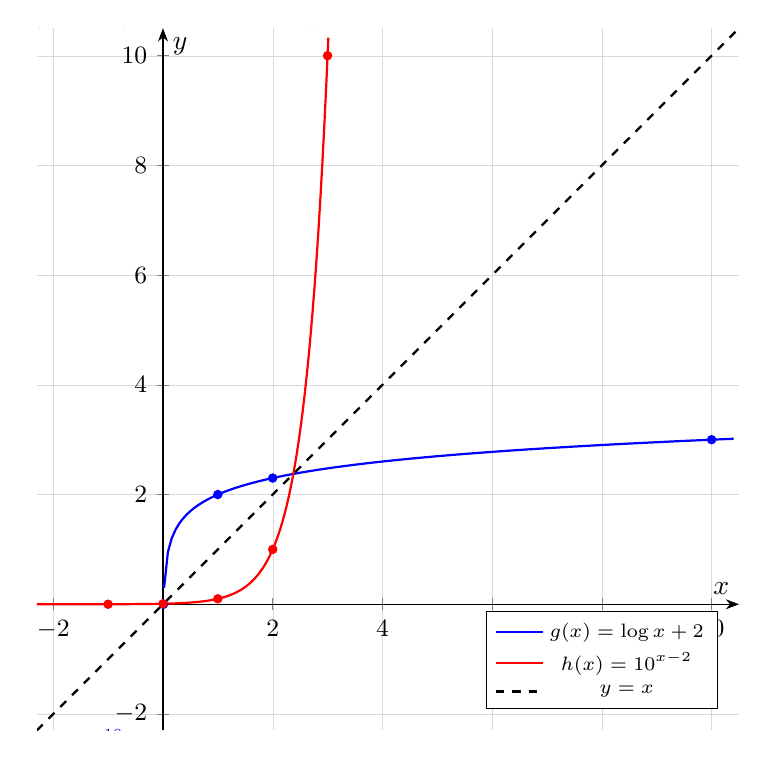
\begin{tikzpicture}
\begin{axis}[
    axis lines = middle,
    xlabel = {$x$}, ylabel = {$y$},
    grid=both,
    grid style={line width=.1pt, draw=gray!30},
    axis line style={-Stealth},
    legend style={font=\scriptsize},
    tick label style={font=\small},
    xmin=-2.3, xmax=10.5, ymin=-2.3, ymax=10.5,
    xtick={-2,0,2,4,6,8,10},
    ytick={-2,0,2,4,6,8,10},
    width=10.5cm, height=10.5cm,
    legend pos=south east,
]
\addplot[domain=0.02:10.4, samples=150, thick, blue] {ln(x)/ln(10)+2};
\addlegendentry{$g(x)=\log x + 2$}
\addplot[domain=-2.3:3.05, samples=150, restrict y to domain=-2.3:10.5, thick, red] {10^(x-2)};
\addlegendentry{$h(x)=10^{x-2}$}
\addplot[domain=-2.3:10.5, samples=2, thick, black, dashed] {x};
\addlegendentry{$y=x$}
\addplot[only marks, mark=*, mark size=1.5pt, blue] coordinates {(0.01,0) (1,2) (2,2.301) (10,3)};
\addplot[only marks, mark=*, mark size=1.5pt, red] coordinates {(-1,0.001) (0,0.01) (1,0.1) (2,1) (3,10)};
\node[anchor=north west, font=\tiny, blue] at (axis cs:-2.2,-2.1) {$g(10^{-10})=-8$ (off-scale, near asymptote)};
\node[anchor=south east, font=\tiny, red] at (axis cs:3,10.3) {$h(4)=100$ (off-scale, continues up)};
\end{axis}
\end{tikzpicture}
\end{document}
